\chapter{Implementierung und Zielsysteme}
\label{cha:Implementierung}
In diesem Kapitel wird die Umsetzung der einzelnen Algorithmen des in Kapitel \ref{cha:konzept} erl�uterten Konzepts mit Hilfe der Software Matlab/Simulink erkl�rt.
F�r einen besseren �berblick zum dem Konzept zeigt die Abbildung \ref{Ablaufdiagramm} ein Ablaufdiagramm des Programms der Bahnplanung.\\

\begin{figure}[H]
	\centering
	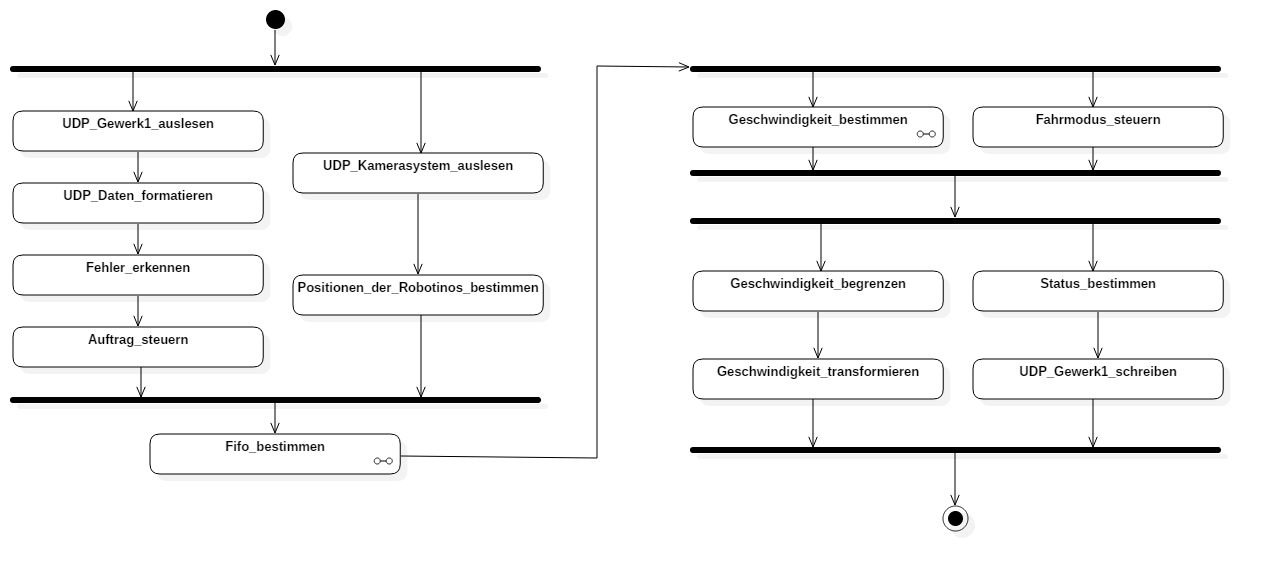
\includegraphics[width=0.9\textwidth]{Bilder/Bahnplanung.png}
	\caption{Ablaufdiagramm Konzept}
	\label{Ablaufdiagramm}
\end{figure}
\noindent
Zun�chst wird der Auftrag der Fertigungsplanung verarbeitet und parallel dazu wir die eigene Position des Robotinos sowie auch die Positionsdaten der anderen Robotinos bezogen. Nachdem die Selbstorganisation durch Wartebereiche abgearbeitet wurde wird das erhaltene Ziel weitergeleitet. Mit dem bekannten Ziel wird der Zielvektor bestimmt. Die Hinderniserkennung l�uft nun gleichzeitig.
Hat der Robotino sein Endziel erreicht kann ein neuer Auftrag abgearbeitet werden.\\
\\Hat ein Robotino zur Zeit keinen Auftrag wird als Ziel die Standby-Position einprogrammiert. Zun�chst wird der Grundalgorithmus zur Zielgebung erl�utert und anschlie�end um die einzelenen Unterpunkte des Konzeptes erweitert.\\

\section{Potentialfeld}
\label{sec:potentialfeld}

\section{Selbstorganisation durch Wartebereiche}
\label{sec:Impl:Selbstorga}
Die in dem Unterkapitel \ref{subsec:Selbstorga} erkl�rte intelligente Selstorganisation wird im folgenden erkl�rt und es wird gezeigt wie der Algorithmus in der Software Simulink umgesetzt wird. \\
\\
Das Ablaufdiagramm in Abbildung \ref{AblaufdiagrammFIFO} stellt den Ablauf des  Algorithmus dar.\\

\begin{figure}[H]
	\centering
	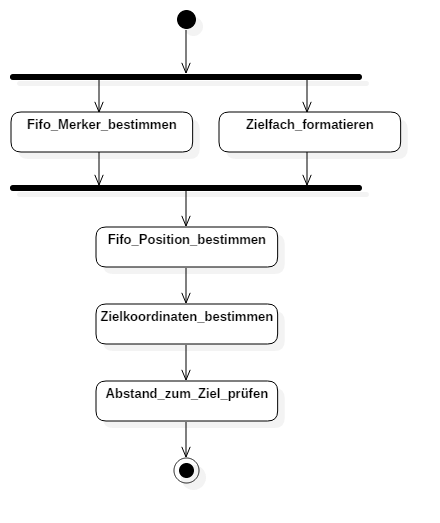
\includegraphics[width=0.4\textwidth]{Bilder/FIFO_Steuerung.png}
	\caption{Ablaufdiagramm der Selbstorganisation}
	\label{AblaufdiagrammFIFO}
\end{figure}
\noindent
\\
Die Positionen der anderen Robotinos werden �ber den 'FIFO Merker' gepr�ft und es wird geschaut ob die anderen Roboter Positionen einnehmen die ein zugeh�riger Warteplatz f�r die Zielstation darstellen.\\
Die Roboterpositionen werden in einem Array der X- Positionen und einem der Y-Postionen gespeichert. Die 12 bestehenden in gleichm��igen Abstand aufgeteilten Wartebereiche k�nnen mit der Formel \ref{equ:wartebereiche} in Zeile 8 des Matlabcodes \ref{Fifomerker} in X-Richtung berechnet werden.\\
\begin{align}
\label{equ:wartebereiche}
  N(n)=round((X(n)-703)/400)+1;
  \end{align}  
Stimmen die X-Positionen der Robotinos mit den Bereichen überein und sind die Y-Positionen am linken Rand des gesamten 'Fabrik' Bereiches, wird der Wartebereich an dem ein Robotino mit einer jedem Robotino spezifischen Nummer belegt.
Damit die Wartebereiche auch in jedem Zyklus wieder neu berechnet werden wird der Merker zunächst auf 0 gesetzt und in jedem Zyklus mit neuen Werten beschrieben.\\

\newpage
\begin{lstlisting}[caption={FIFO Merker},label=Fifomerker,basicstyle=\small]
function [FifoArray1,StationArray1,LadeArray1]= fcn(Robbi,FifoArray,LadeArray)
X=[Robbi(1) Robbi(4) Robbi(7) Robbi(10)];
Y=[Robbi(2) Robbi(5) Robbi(8) Robbi(11)];
FifoArray1=zeros([1 12]);
FifoArray1=FifoArray(1:12);
N=zeros([1 5]);
for n= 1 : 1 : 4
        N(n)=round((X(n)-703)/400)+1; % Berechnung in welchem Fifo der Roboter sich befinde
elseif (Y(n)<450 && (X(n)>100 && X(n)<5250)&& N(n)<=12 && N(n)>0)
        for i=1:12
            if FifoArray1(i)==n
                FifoArray1(i)=0;
            end
        end
            FifoArray1(N(n))=n;
          ...
          ...
end
\end{lstlisting}
Auch die Belegung der Stationen wird mit dem selben Algorithmus berechnet. Einzig die Bereichsabfrage �ndert sich und die Formel \ref{equ:wartebereiche} f�r die Berechnung der Belegung. Hierbei �ndert sich allerdings nur die Unterteilung und der Offset der Formel.\\
Die Merkerwerte werden in einem Stateflowdiagramm weiterverarbeitet. Die Eingänge des Stateflowdiagramms sind die Auftragsdaten, die Merkerdaten, und die genauen Positionsdaten des Robotinos aus Beobachter und Kamerawerten.
Damit das System die Wartepositionen der zugeh�rigen Zielstationen f�r die Zuweisung verwendet wird die Formel \ref{equ:ersterfifo} verwendet. Die 12 Wartebereiche k�nnen so explizit den 8 Stationen zugeordnet werden. Zwei Stationen teilen sich jeweils drei Wartebereiche.
\begin{align}
\label{equ:ersterfifo}
 &ersterFifo=floor(Zielstation/2)\cdot3+2 \cdot mod(Zielstation,2)+1\\
 &zweiterFifo=floor(Zielstation/2)\cdot 3+1+1\\
 &dritterFifo=floor(Zielstation/2)\cdot 3+2-2\cdot mod(Zielstation,2)+1
  \end{align} 
Ist der erste Bereich belegt wird der zweite Bereich abgefragt ist dieser belegt wird der Dritte abgefragt. Sind alles drei Bereich belegt gibt das Stateflow diagramm den h�chsten Wert aus. Beim h�chsten Wert wird die Standbyposition als Ziel einprogrammiert.\\
\\

Wird im n�chsten Zyklus der n�chst kleinere Wartebereich frei so wird dieses als Ziel angefahren. 
In dem Fall wenn ein anderer Robotino den ersten Wartebereich verl�sst und zur Zielstation f�hrt besteht ein Sonderfall. Da die Strecke zwischen den beiden Punkten ca. zwei Meter betr�gt dauert diese Fahrt mehrere Zyklen. Damit ein dahinter stehender Robotino in dem Moment nicht auch direkt die Station anf�hrt, weil alle anderen Bereiche frei sind, wird eine weitere Position abgefragt. Die Stationsbelegung wird abgefragt. 
Die Station wird erst wieder freigegeben wenn sie im Stationsmerker nicht mehr belegt ist.\\

\section{Bekannte Hindernisse}

F�r eine verbesserte Kollisionsvermeidung wurde das Ausweichman�ver, wie in Unterkapitel \ref{subsec:bekannt} bereits erkl�rt, verwendet. Die Aufgabe des Man�vers ist es den Zielvektor des Robotinos so zu verändern, dass er einem sich im Weg befindenden Robotino mit einem gr��eren Abstand ausweicht.
Es werden die Position des Robotinos ben�tigt sowie auch die Positionen der anderen Robotinos, die St�rpositionen. Dar�ber hinaus ben�tigt das Man�ver den Zielvektor.\\
Zun�chst wird analysiert in welchem Winkel die St�rpositionen sich zum Zielvektor befinden. Liegt ein anderer Robotino innerhalb von \ang{30} zum Zeilvektor wird ein Ausweichwinkel berechnet. 
\begin{align}
\label{Ausweichwinkel}
Ausweich(1,i)=+asin(Abstand(2,i)/Hyp)-pi/2
\end{align}
Der erste Wert des Ausweichs-Array aus Formel \ref{Ausweichwinkel} ist der Ausweichwinkel. �ber eine Trigonometrische Funktion wird der genaue Winkel des Zielvektors zum Ziel ausgerechnet und \ang{90} addiert.
Solange eine St�rposition innerhalb der \ang{30} liegen bleibt der Ausweichwinkel erhalten. Ist der im Weg liegende Roboter weitgenug umfahren wird der originale Zielvektor einprogrammiert.

\section{Unbekannte Hindernisse}
 
Unbekannte Hindernisse werden nur mit Hilfe der 9 verbauten Infrarotsensoren erkannt. Zyklisch werden diese Sensoren abgefragt. Detektiert einer der Sensoren ein Hindernis wird zun�chst �berpr�ft an welcher Position relativ zur Roboterausrichtung sich das Hindernis befindet. Der Ablauf wird im Code \ref{infra} dargestellt:\\
\begin{lstlisting}[caption=Infraroterkennung,label=infra,basicstyle=\small]
for x=1:9
 if  (isnan(IRDaten(x))==0) && (IRDaten(x) <= 150)
  IRWerte(1,x)=cos(((x-1)*40*pi/180)+RobPos(3))*(IRDaten(x)+200)+RobPos(1);
  IRWerte(2,x)=sin(((x-1)*40*pi/180)+RobPos(3))*(IRDaten(x)+200)+RobPos(2);
 else
  IRWerte(1,x)=NaN;
  IRWerte(2,x)=NaN;
 end
end
\end{lstlisting}
